
{\sl This fieldstone was developed in collaboration with Job Mos}.

From \cite{dohu}. In order to illustrate the behavior of selected mixed finite elements in the solution 
of stationary Stokes flow,  we consider a two-dimensional problem 
in the square domain $\Omega=[0,1]\times[0,1]$, which possesses a closed-form analytical 
solution. The problem consists of determining the velocity field ${\bm v} = (u,v)$ and the 
pressure $p$ such that 
\[
-\nu \Delta {\bm v} + {\bm \nabla} p = {\bm b}  \quad\quad {\rm in} \; \Omega
\]
\[
{\bm \nabla} \cdot {\bm v} = 0 \quad\quad {\rm in} \; \Omega
\]
\[
{\bm v}={\bm 0} \quad\quad {\rm on} \; \Gamma
\]
where the fluid viscosity is taken as $\nu=1$. 


\fbox{
\parbox{10cm}{{\bf features}
\begin{itemize}
\item $Q_1\times P_0$ element \index{$Q_1 \times P_0$}
\item incompressible flow
\item penalty formulation \index{penalty formulation}
\item Dirichlet boundary conditions (no-slip)
\item direct solver 
\item isothermal \index{isothermal}
\item isoviscous \index{isoviscous}
\item analytical solution \index{analytical solution}
\end{itemize}
}}

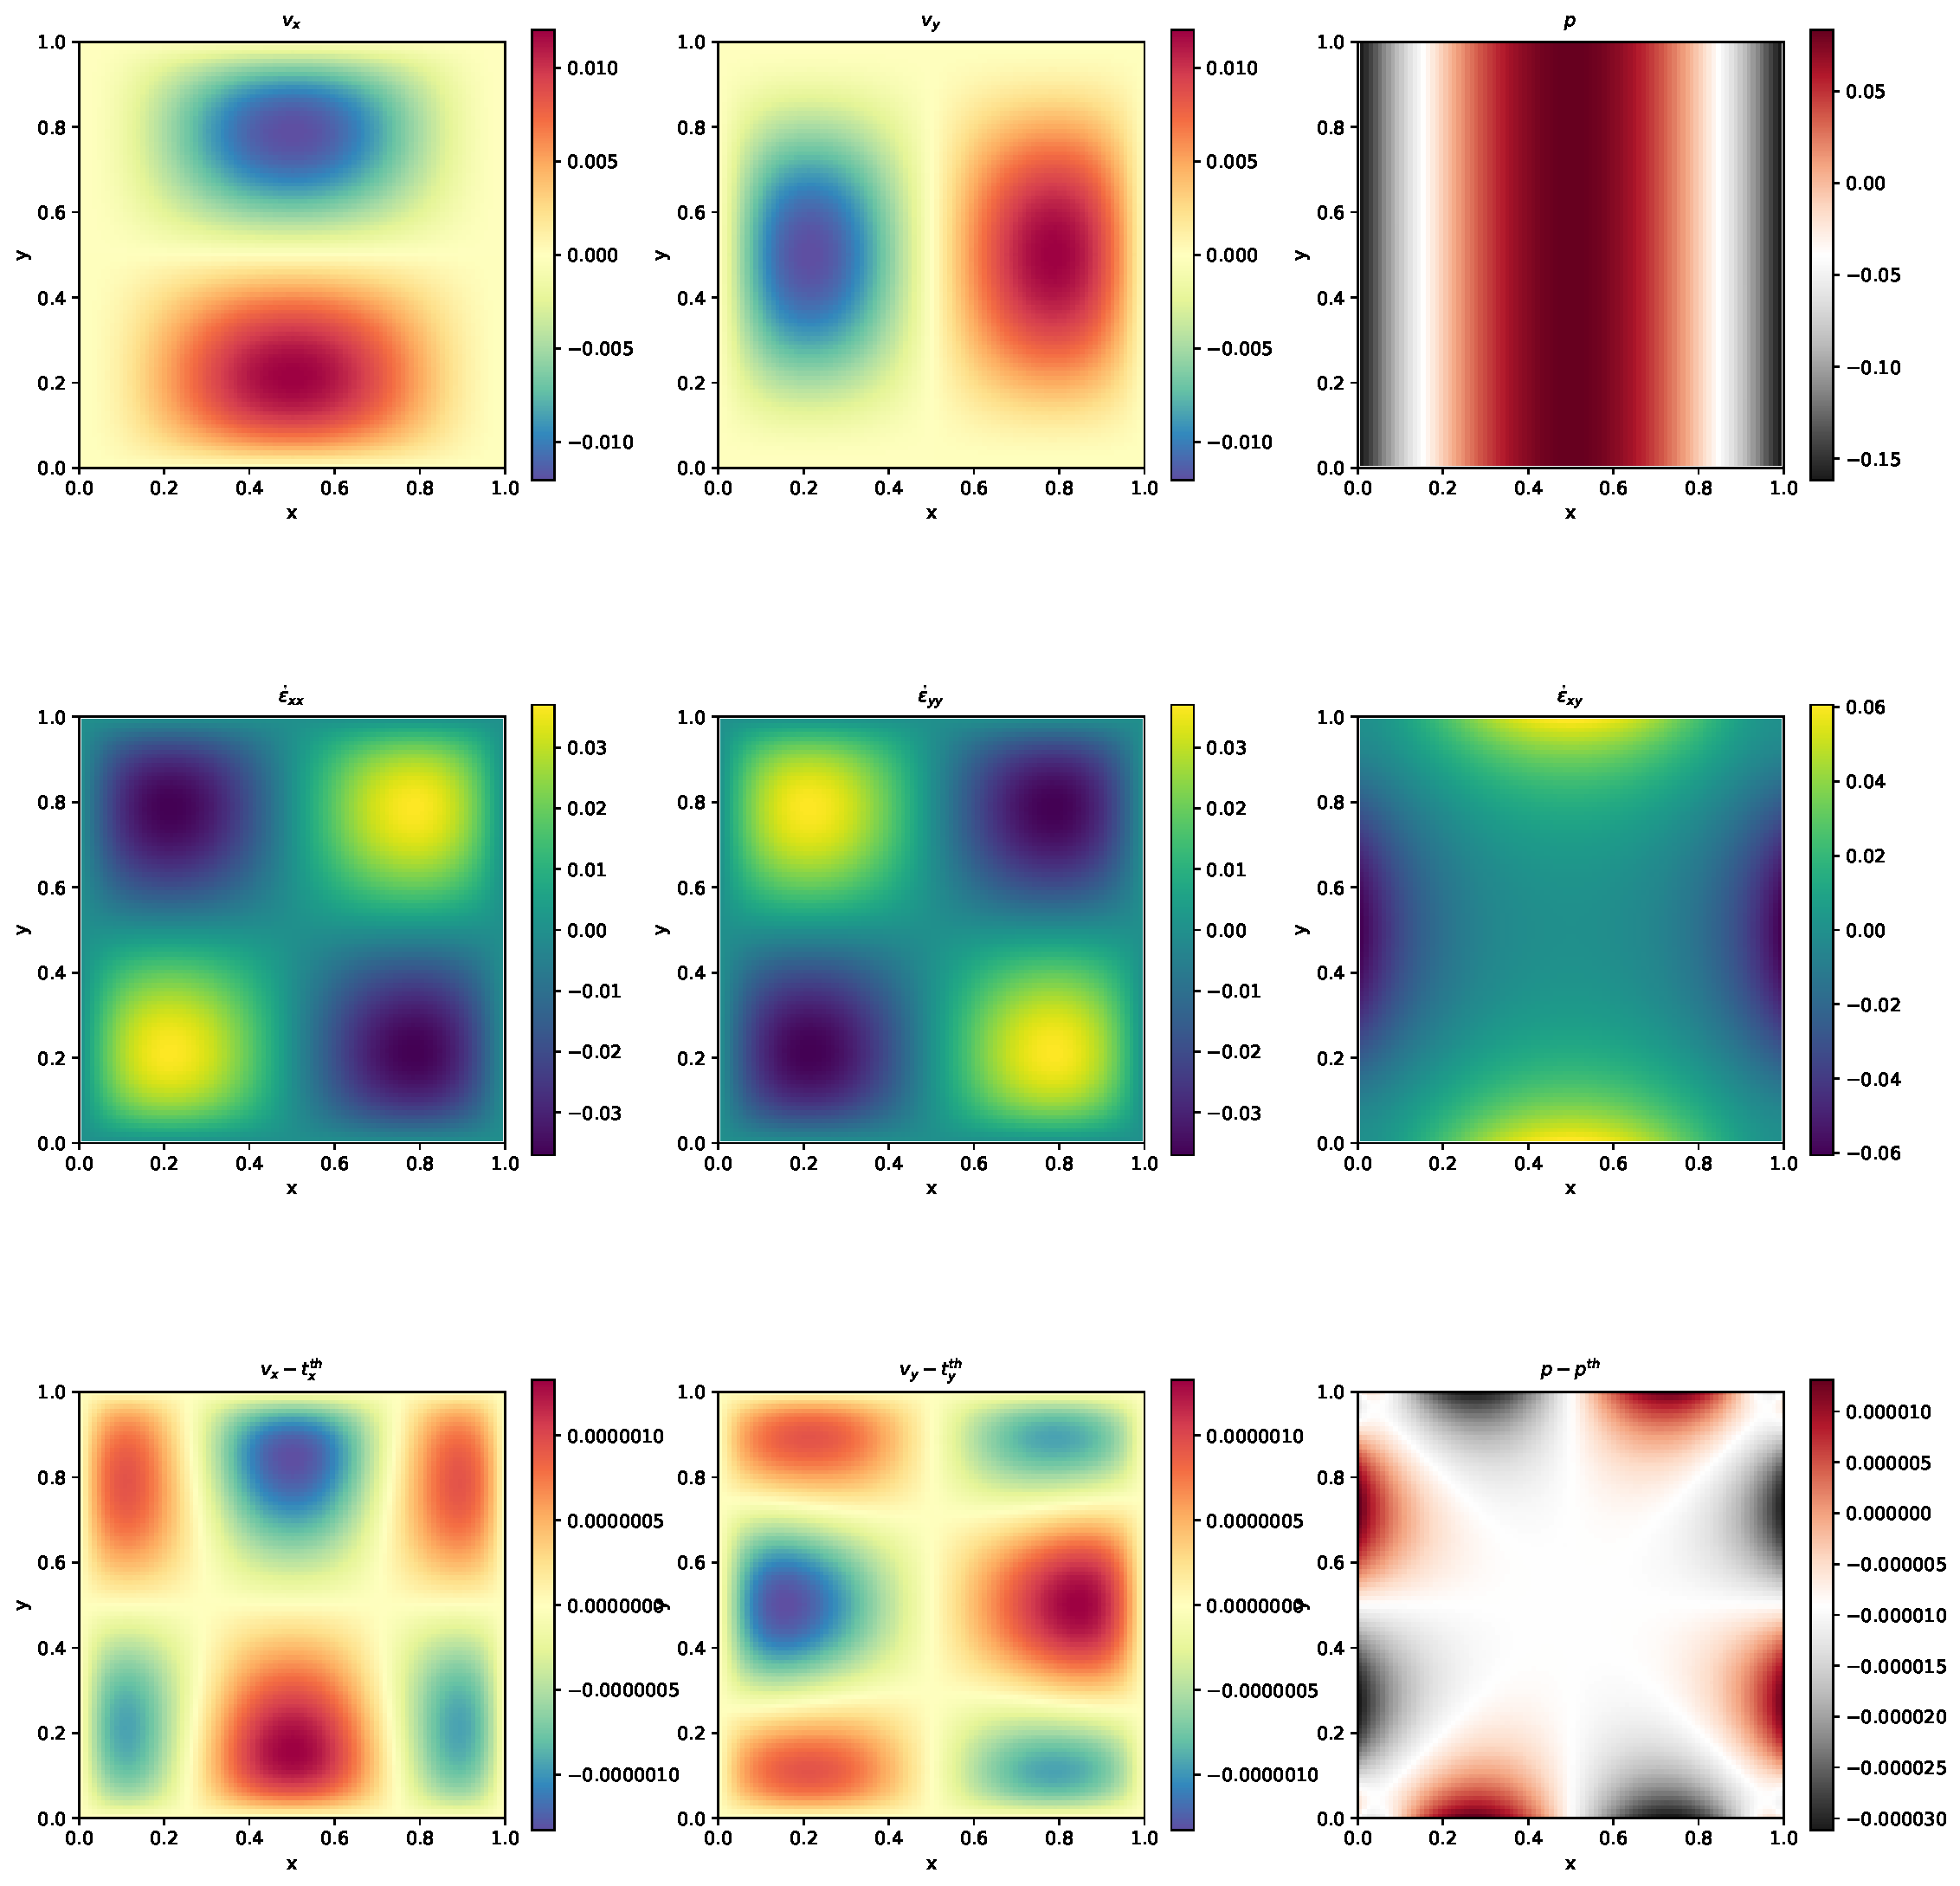
\includegraphics[width=16cm]{python_codes/fieldstone_01/solution.pdf}

\begin{center}
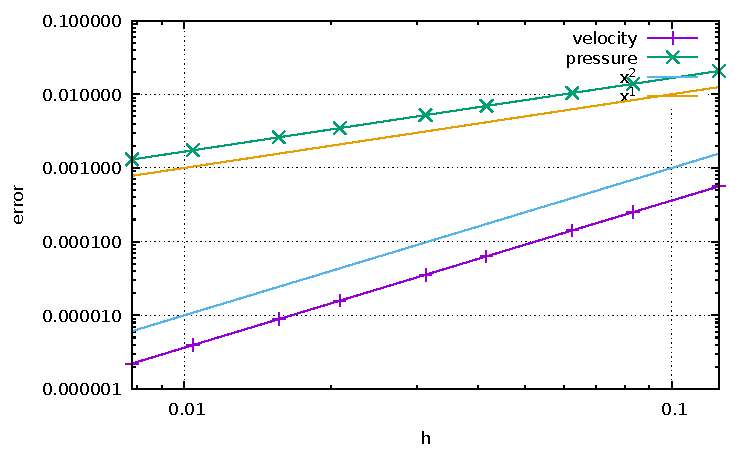
\includegraphics[width=12cm]{python_codes/fieldstone_01/errors.pdf}\\
Quadratic convergence for velocity error, 
linear convergence for pressure error, as expected.
\end{center}

ToDo:

pressure normalisation?

different cmat, a la schmalholz

To go further:
\begin{enumerate}
\item make your own analytical solution
\end{enumerate}
